\chapter{Literature and Technology Survey}
\label{chap:technology survey}

\section{Amazon Alexa and Google Assistant}
In the domain of voice-activated smart speakers, the market is primarily led by two ecosystems: the Amazon Echo range and the Google Home series. Both systems utilise virtual assistants---Alexa and Google Assistant, respectively---which are activated via a specific wake command, such as ``Alexa'' or ``Hey Google''. These platforms allow third-party developers to create bespoke applications, referred to as `skills' in the Amazon ecosystem and `actions' within Google's, which can be invoked by users to extend the device's functionality.

\begin{figure}[H]
\centering
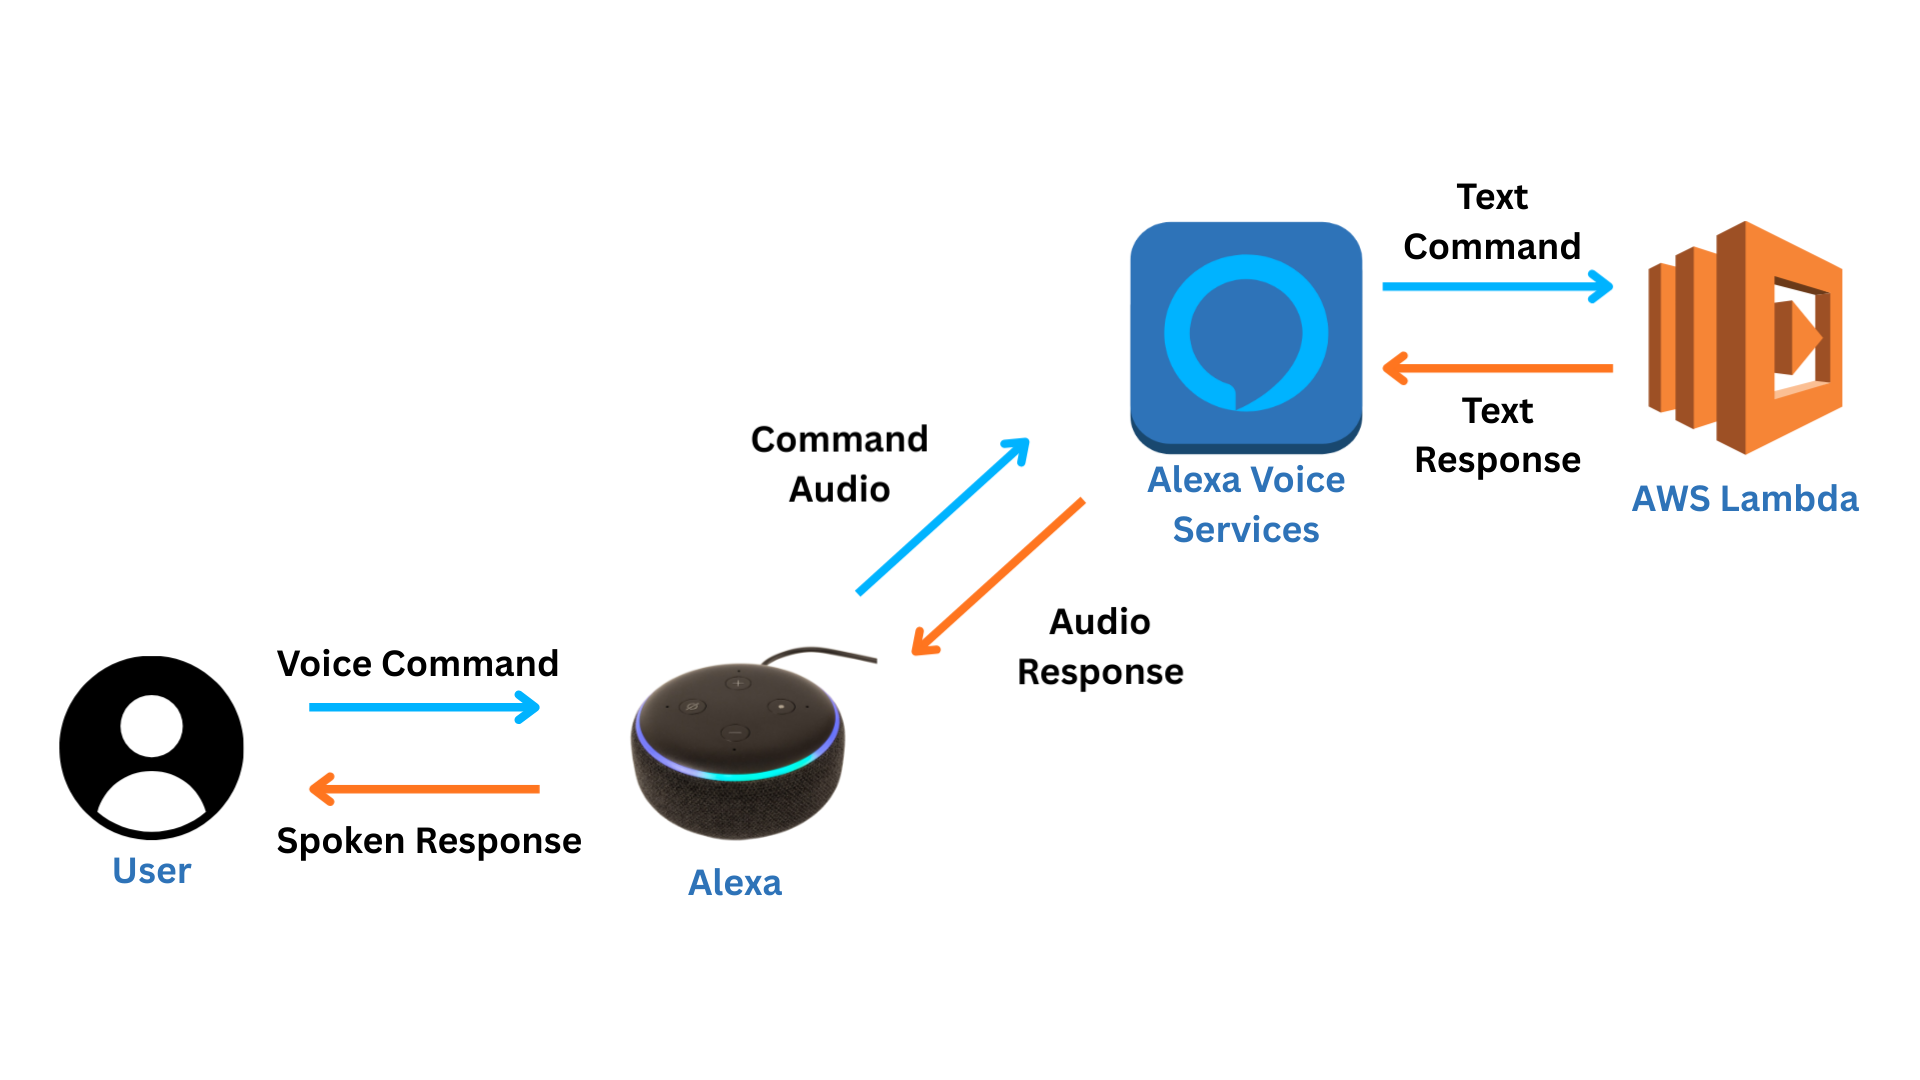
\includegraphics[width=0.9\linewidth]{./images/Voice Command.png}
\caption{Visualisation of the Request-Response Cycle within an Alexa Skill}
\label{fig:alexa-diagram}
\end{figure}

Data provided by Statista Consumer Insights indicates that Amazon maintains a significantly larger market share compared to Google in the smart speaker sector (\autoref{fig:SmartSpeakerChart}). Consequently, the Amazon Alexa platform represents a more strategic target for development, offering a broader potential user base for the deployment of new predictive tools.

\begin{figure}[H]
    \centering
    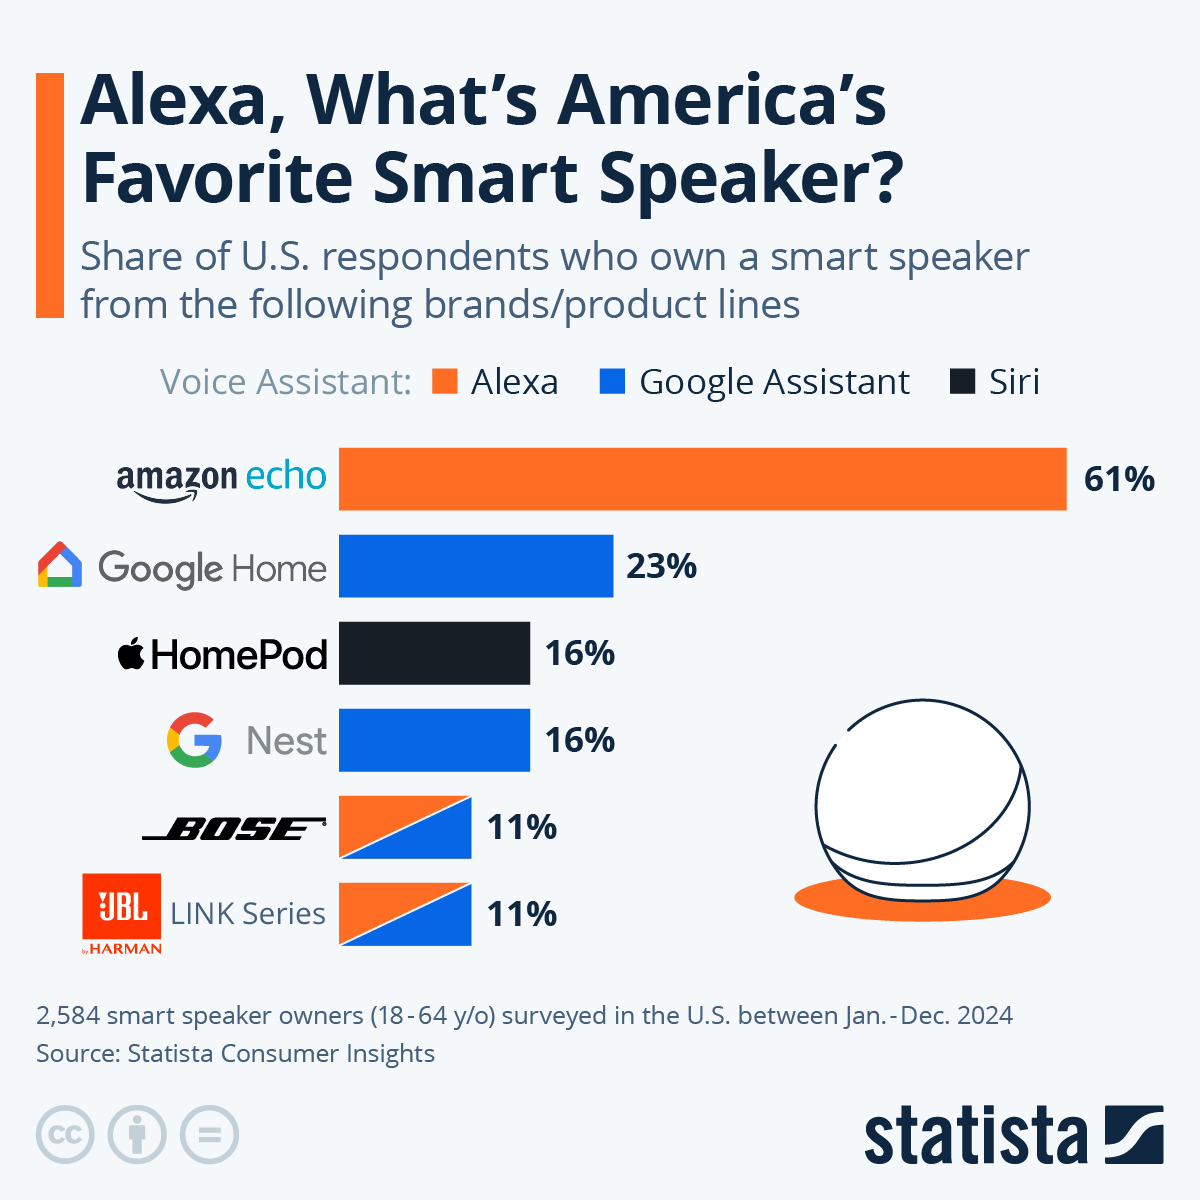
\includegraphics[width=0.75\linewidth]{./images/SmartSpeakerChart.png}
    \caption{Market share of smart speaker ownership amongst adults.\cite{statista_smartspeaker}}
    \label{fig:SmartSpeakerChart}
\end{figure}

\section{Platform Selection and Technical Constraints}
The development of an Alexa skill is facilitated through the Amazon Developer Console, a cloud-based environment used for the configuration and management of voice interactions. While the platform supports various programming languages, Python and JavaScript are provided as the primary languages with native \gls{sdk} (Software Development Kit) support. Hosting typically involves AWS Lambda, a serverless computing platform, though developers may also provision custom endpoints for local execution and debugging.

A critical technical constraint was identified during the evaluation of the Google Home ecosystem. Google has recently deprecated `conversational actions' in favour of `app actions', as documented in the Assistant Developer documentation\cite{google_sunset}. This shift implies that new Google Assistant developments must be tethered to a corresponding Android application. Given that this project is intended to function as a standalone voice service without a prerequisite mobile application, the sunsetting of conversational actions effectively precludes Google Home as a viable launchpad. Therefore, the decision was made to proceed exclusively with the Amazon Alexa platform.

\section{Language Selection and Development Environment}
Selecting an appropriate primary programming language is a critical architectural decision, as the choice directly influences the availability of documentation, pre-built libraries, and the overall complexity of the implementation. A language with insufficient support for machine learning would necessitate the manual development of boilerplate code, increasing the risk of project delays. Conversely, a language with an excessively steep learning curve could impede the preliminary stages of development. Therefore, a balance between technical capability and development efficiency must be established.

Following a comparative evaluation of the supported environments for Alexa Skill development, Python was identified as the optimal language for this project. Python is widely regarded as the industry standard for machine learning and data science, offering an extensive ecosystem of libraries that abstract complex mathematical operations and reduce manual implementation. The language's syntax and conventions further contribute to code readability and long-term maintainability. The following libraries were identified as essential to the project's success:

\begin{itemize}
\item \textbf{NumPy:} This library facilitates high-performance operations on multi-dimensional array objects. NumPy is reported to be significantly more efficient than standard Python lists, which is crucial when processing the large datasets typical of machine learning workflows. \cite{numpy_site}
\item \textbf{pandas:} This provides a high-performance DataFrame object for structured data manipulation. It includes integrated tools for reading and writing data in various formats, such as CSV, and offers a powerful engine for aggregating and merging disparate datasets. \cite{pandas_site}
\item \textbf{scikit-learn:} A comprehensive suite of machine learning tools, including various classification algorithms, utilities for data splitting (training and testing sets), and metrics for evaluating model performance. \cite{sklearn_site}
\end{itemize}

\section{The Dataset}
To develop a machine learning model with predictive power beyond stochastic chance, a robust set of features must be identified and obtained. Within the context of a Valorant match, data granularity ranges from high-level outcomes, such as the overall winner, to round-specific metrics, such as individual elimination counts. This spectrum of data allows for an iterative development approach: a model may be initialised using a small subset of primary features, with more complex, derived features integrated during later stages of implementation.

Two primary methods for acquiring a suitable dataset were evaluated: manual creation via web-scraping or the utilisation of a pre-existing dataset. The manual creation of a dataset would require the development of a bespoke web-scraper to request the HTML content of match results from historical VCT data since 2021. For instance, extracting team names from a repository such as VLR.gg \cite{vlr_gg} would involve querying the DOM using feature unique CSS selectors, such as \texttt{\#wf-title-med}. While this method offers maximum control over the data schema, the process of extraction, standardisation, and anomaly detection is substantially time-consuming.

Conversely, the use of an existing dataset requires a rigorous assessment of feature richness and data integrity. It is essential to ensure that the dataset captures the underlying relationships between match variables and the final outcome without introducing multicollinearity---a state where redundant features communicate identical information. Furthermore, any external data must be used in strict accordance with the original author's licensing and copyright terms.

Given the significant time investment required for manual scraping, the acquisition of a comprehensive, pre-existing dataset was prioritised. A suitable dataset was identified and sourced from a repository on Kaggle \cite{ryanluong_dataset}. \autoref{tab:key-dataset-features} provides a data dictionary of the critical features extracted for this project, while the following subsection details their predictive significance.

\subsection*{Dataset Features}
Features within the dataset are categorised into two primary domains: player-level and team-level metrics. Player-level features, such as `Average Combat Score (ACS)', provide an indication of the individual technical proficiency of the team's constituents. Team-level features, such as `Attacker Score', offer high-level insights into team dynamics and situational performance. In the following table, features denoted with `X' represent data collected for both competing teams (Team A and Team B) respectively.

\begin{table}[H]
    \centering
    \small
    \begin{tabularx}{\linewidth}{|>{\raggedright\arraybackslash}p{3cm}|>{\raggedright\arraybackslash}p{5cm}|>{\raggedright\arraybackslash}X|}
        \hline
        \textbf{Feature} & \textbf{Definition} & \textbf{Predictive Utility} \\ \hline
        Team X & The name of a competing team. & Acts as a primary key for grouping historical performance data. \\ \hline
        Map & The game map in which the match took place. & Facilitates the derivation of map-specific win rates and performance biases. \\ \hline
        Team X Score & Total rounds won by a team. & Used to determine the match winner and calculate rolling performance metrics (e.g., win percentage over $n$ matches). \\ \hline
        Team X Attacker / Defender Score & Rounds won while on the attacking or defending side. & Used to assess side-specific proficiency and map-side advantage. \\ \hline
        KAST & Percentage of rounds featuring a kill, assist, survival, or trade. & Measures a player's overall contribution to team-oriented play. \\ \hline
        First Kills / Deaths & Frequency of a player being the first to eliminate or be eliminated in a round. & Indicates round-opening aggression and survivability; critical for early-round advantage. \\ \hline
        Average Combat Score & Aggregate score based on damage, kills, assists, and multi-kills. & Serves as a weighted proxy for individual mechanical performance. \\ \hline
        Pistol Won & A binary flag indicating the winner of the initial round of each half. & Acts as a lead indicator for match momentum and subsequent round economic advantage. \\ \hline
    \end{tabularx}
    \caption{Key Dataset Features and their Predictive Significance}
    \label{tab:key-dataset-features}
\end{table}

\section{Exploring Machine Learning Approaches}
"Machine learning (ML) is a field of study in artificial intelligence that is concerned with the development and study of statistical algorithms that can learn from data and generalise to unseen data and thus perform tasks without explicit instructions" \cite{Koza1996}.

Machine learning is used in a vast amount of people's lives every month, perhaps without them even knowing it. For example, Facebook—the world's 2nd most popular social network by number of users \cite{BacklinkoTeam2025}—"uses machine learning to generate the estimated action rate and the ad quality score used in the total value equation" \cite{Facebook2020}. What this means is that possible adverts that might be shown to the user are scored, by a machine learning algorithm, as to how successful they might be in influencing that users decision, as well as the quality of the advert. Facebook now has 3.07 billion monthly active users as of October 2025, and did have 3.65 billion in 2024 \cite{NaveenKumar2025}, which is a lot of people being exposed to ML via only one platform.

Recently, bookmakers have also shifted towards using predictive machine learning models to generate the odds of a specific outcome, which they can then use to sell bets to customers \cite{RhysGregory2025}. This is the most similar example of ML being used in industry to my project.

To successfully accomplish the aim that I have set for myself, some form of machine learning approach will need to be implemented. There is a vast amount of different training and prediction algorithms available to me, all of which are better suited to different tasks. ML algorithms fall under 4 categories, supervised, unsupervised, semi-supervised, and reinforcement learning \cite{Sarker2021}.

\subsection*{Supervised Learning}
Supervised learning is the process of teaching a machine by example. The algorithm is provided with a dataset where the human knows the correct outputs for the set of inputs. The machine makes predictions using the provided data, and is corrected when wrong, until the algorithm has been refined enough for there to be a high degree of \gls{accuracy}. This approach is well suited to predicting or classifying new, unseen data based off of the patterns recognised from the labelled training data. However, supervised learning is not as good at discovering new patterns, only at predicting based off of existing ones. Also, it requires a sufficiently large, accurately labelled dataset, which is time consuming and expensive to procure/produce. \cite{SupervisedLearning}

\begin{figure}[H]
    \centering
    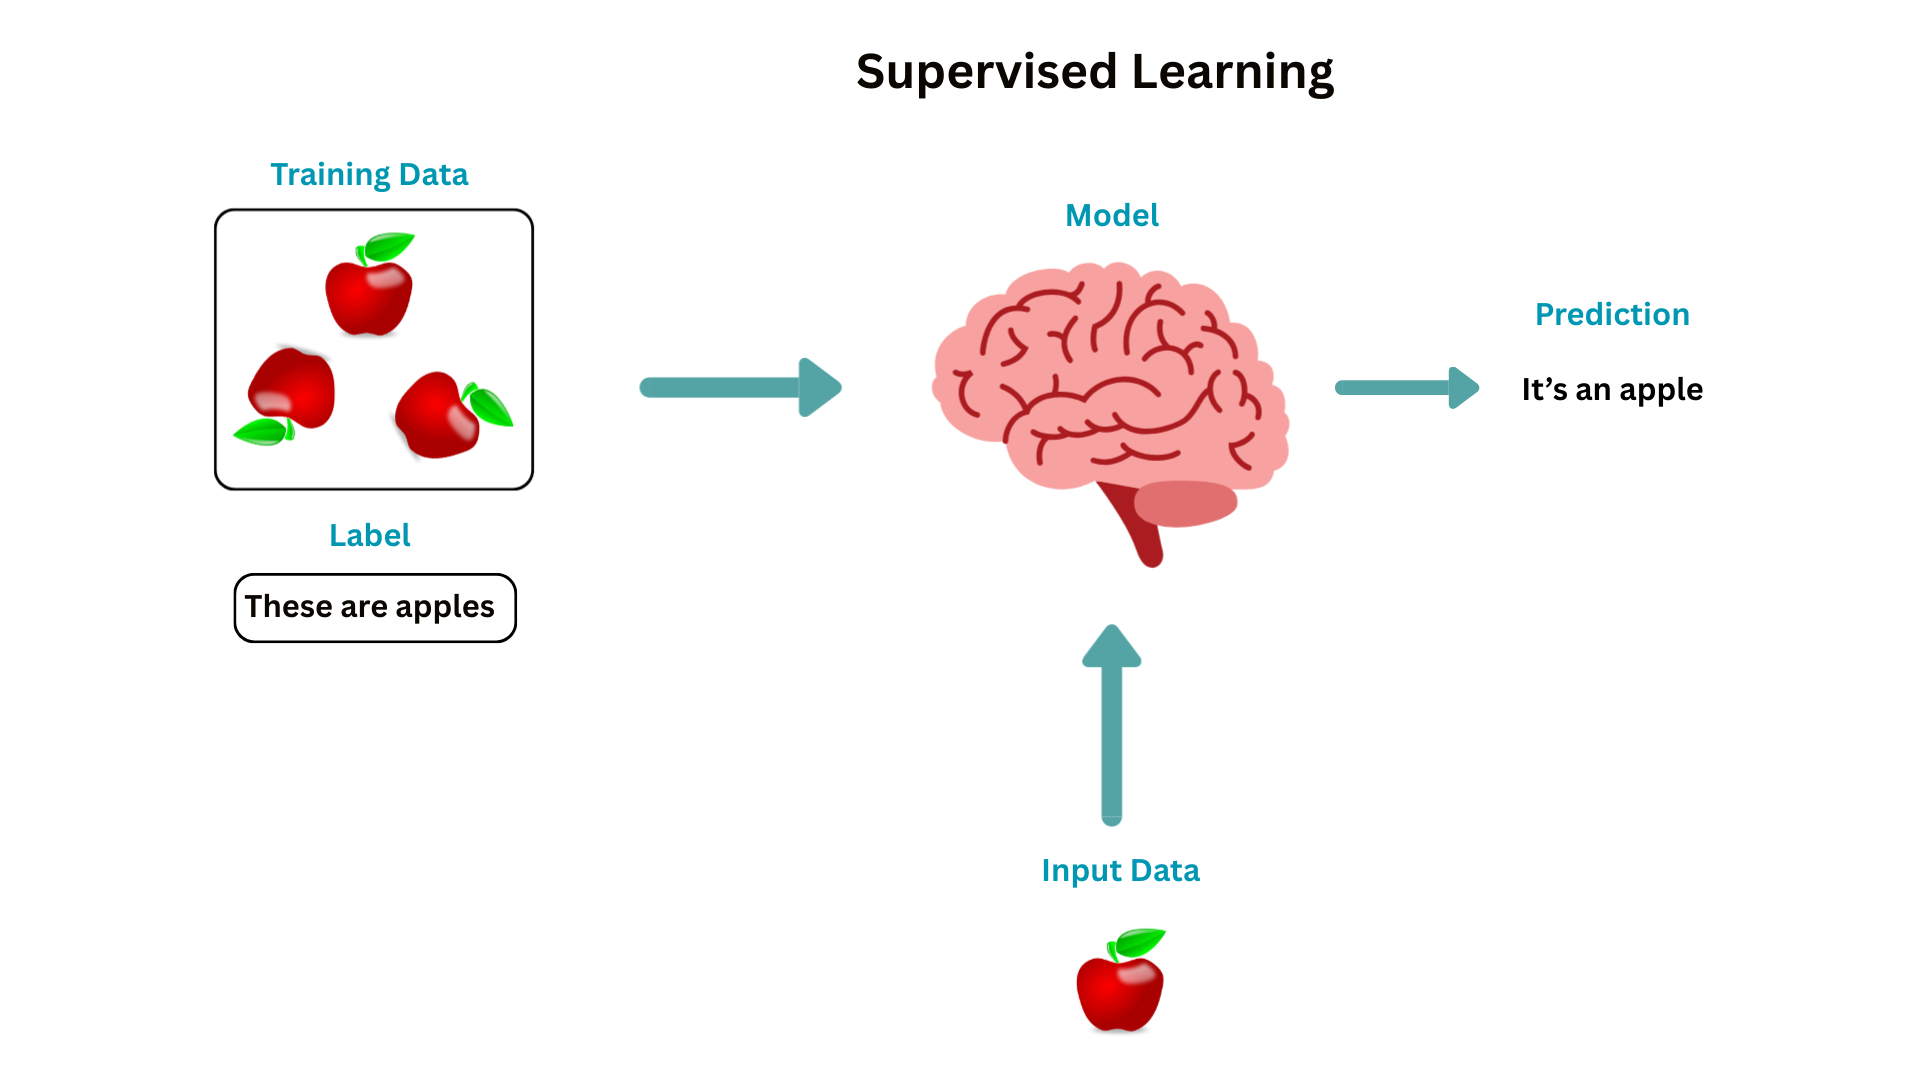
\includegraphics[width=1\linewidth]{./images/Apple (1).png}
    \caption{Depiction of Supervised Learning}
    \label{fig:supervised-learning}
\end{figure}

\subsection*{Unsupervised Learning}
Unsupervised learning is where the machine studies large, unlabelled datasets to pick out patterns and organise the data in some way. There is no correction taking place from the human, since the data is not labelled. Given a large set of data, and without human input, unsupervised learning algorithms will discover hidden patterns or data groupings automatically. Unsupervised learning lends itself nicely to exploratory data analysis, being able to collate data points into separate 'clusters', or to identify outliers and anomalies from a dataset. Usually, the datasets used are acquired 'cheaply', such as web-crawling, where there is an enormous quantity of data available without a large cost. Unsupervised learning is however less useful when a precise output is required. Due to the nature of being trained on unlabelled data, the machine doesn't know what right answers are, only outputting the patterns it sees, in many cases being categories that are not meaningful or relevant \cite{TeamDigitalDefynd:online}.

\begin{figure}[H]
    \centering
    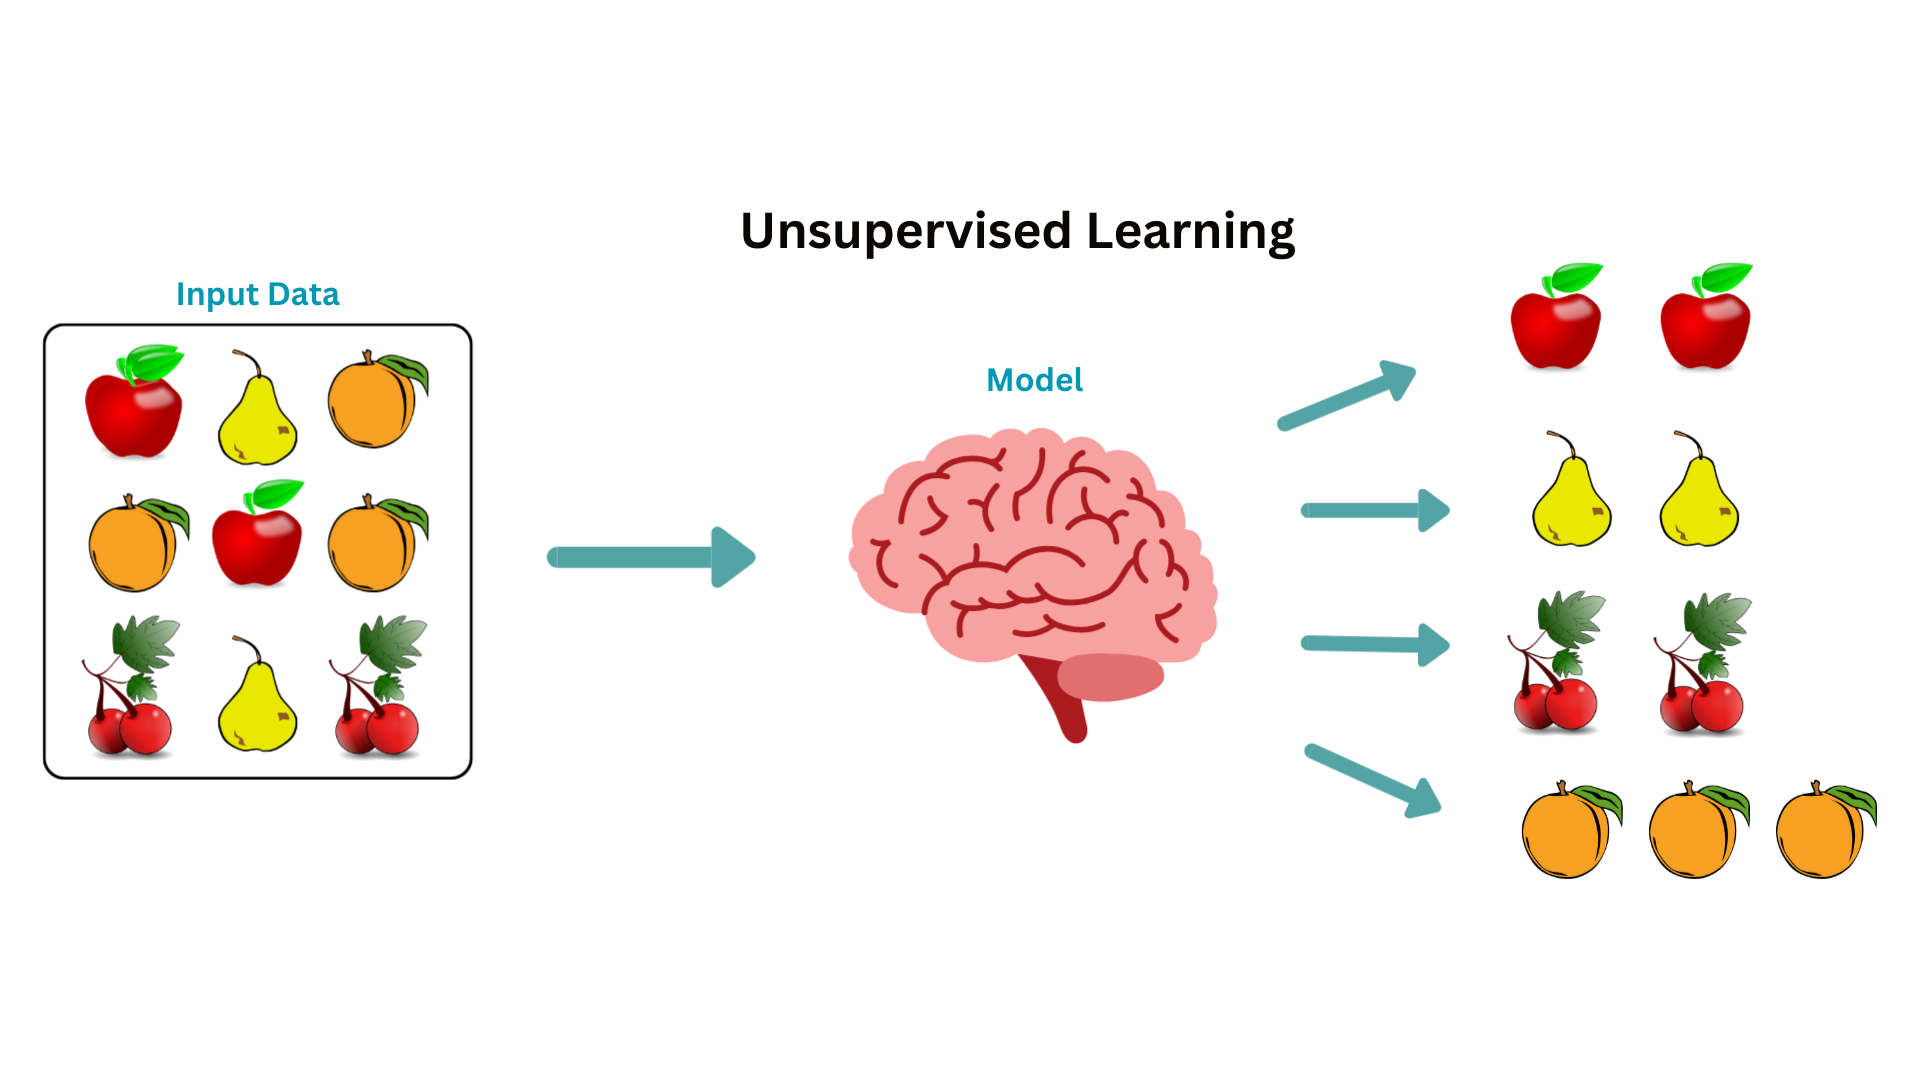
\includegraphics[width=1\linewidth]{./images/Apple.png}
    \caption{Depiction of Unsupervised Learning}
    \label{fig:unsupervised-learning}
\end{figure}

\subsection*{Semi-supervised Learning}
Semi-supervised learning is an approach that combines supervised and unsupervised learning by using both labelled and unlabelled datasets. Semi-supervised learning is commonly utilised for the same contexts as supervised learning models; however semi-supervised models also harness unlabelled data when training, alongside the existing labelled data. It is useful for machine learning tasks where a sufficient quantity of labelled data is prohibitively difficult or expensive to obtain, but a large quantity of unlabelled data isn't. Both supervised and unsupervised learning would underperform in such a situation. Semi-supervised learning is less efficient than its already mentioned counterparts when enough labelled data can be gathered to use supervised learning—in which case results will be better due to the correction taking place—or when there is a severe lack or inability to gather labelled data, in which case unsupervised learning would be used. \cite{DaveBergmann}

\subsection*{Reinforcement Learning}
Finally, reinforcement learning (RL) is where an 'agent' will, through trial and error, learn to maximise its 'reward' by making certain decisions. In contrast to supervised and unsupervised learning, RL requires a dataset that consists of state-action-reward sequences. The data points are arranged into an environment for the machine to interact with—where states have transitions to other states—and there is a set goal for the machine to aim for. Initially, the machine will choose random actions from the predefined set available, and it will receive feedback on how each action contributed towards making it closer to the goal. Over time, the machine will assign weights to the actions, proportional to the size of the reward that it received for completing that action. This will lead to the machine choosing, at each time step, the actions that it has been told are the best ones. RL is a good choice for tasks that involve sequential decision making to maximise a long-term cumulative reward. For example, teaching a machine to play games, or to learn dexterity. RL is less suited when tasks don't have clearly defined rewards, and shouldn't be used for tasks with potential danger involved \cite{Hoda2020}.  RL has been used for many different tasks, such as teaching a machine to play Go\footnote{An overview of Go: \url{https://en.wikipedia.org/wiki/Go_(game)}} from scratch, by playing against itself for 40 days. This model was called AlphaGo Zero, and it was able to outperform the previous Go AI that famously beat the world number one Ke Jie, and Lee Sedol \cite{silver2017mastering, lee2016human}.

\begin{figure}[H]
    \centering
    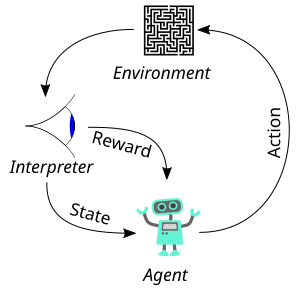
\includegraphics[width=0.5\linewidth]{./images/Reinforcement_learning_diagram.png}
    \caption{Depiction of Reinforcement Learning}
    \label{fig:reinforcement-learning}
\end{figure}

\begin{table}[!ht]
    \begin{tabular}{|l|>{\raggedright\arraybackslash}m{5cm}|>{\raggedright\arraybackslash}m{5cm}|}
        \hline
        \textbf{Approach} & \textbf{Pros} & \textbf{Cons} \\ 
        \hline

        \textbf{Supervised} &
        \vspace{4pt}\begin{itemize}[leftmargin=*,topsep=2pt,partopsep=0pt,parsep=0pt,itemsep=1pt]
            \item Easier to evaluate (since inputs are labelled)
            \item Well-established algorithms
        \end{itemize}\vspace{4pt} &
        \vspace{4pt}\begin{itemize}[leftmargin=*,topsep=2pt,partopsep=0pt,parsep=0pt,itemsep=1pt]
            \item Requires large amounts of labelled data
            \item May over-fit
        \end{itemize}\vspace{4pt} \\ \hline

        \textbf{Unsupervised} &
        \vspace{4pt}\begin{itemize}[leftmargin=*,topsep=2pt,partopsep=0pt,parsep=0pt,itemsep=1pt]
            \item Works without labelled data
            \item Can discover hidden patterns
        \end{itemize}\vspace{4pt} &
        \vspace{4pt}\begin{itemize}[leftmargin=*,topsep=2pt,partopsep=0pt,parsep=0pt,itemsep=1pt]
            \item Hard to evaluate objectively
            \item Patterns may not be meaningful
        \end{itemize}\vspace{4pt} \\ \hline

        \textbf{Semi-supervised} &
        \vspace{4pt}\begin{itemize}[leftmargin=*,topsep=2pt,partopsep=0pt,parsep=0pt,itemsep=1pt]
            \item Uses both labelled and unlabelled data
            \item Efficient for large datasets
        \end{itemize}\vspace{4pt} &
        \vspace{4pt}\begin{itemize}[leftmargin=*,topsep=2pt,partopsep=0pt,parsep=0pt,itemsep=1pt]
            \item Requires careful tuning
            \item Depends on distribution of unlabelled data
        \end{itemize}\vspace{4pt} \\ \hline

        \textbf{Reinforcement} &
        \vspace{4pt}\begin{itemize}[leftmargin=*,topsep=2pt,partopsep=0pt,parsep=0pt,itemsep=1pt]
            \item Learns via interaction and feedback
            \item Good for sequential decision-making
        \end{itemize}\vspace{4pt} &
        \vspace{4pt}\begin{itemize}[leftmargin=*,topsep=2pt,partopsep=0pt,parsep=0pt,itemsep=1pt]
            \item Computationally expensive
            \item Requires well-designed reward function
        \end{itemize}\vspace{4pt} \\ \hline
    \end{tabular}
    \caption{Pros and cons of each machine learning approach.}
    \label{tab:MLProsAndCons}
\end{table}

\noindent In addition, by comparing and contrasting these machine learning paradigms' optimal use cases and drawbacks, I have further reinforced the conclusion that supervised learning is the best approach to pursue further. This is due to the fact that the datasets available on the internet containing information about past Valorant professional matches are all going to be labelled, as the games have already taken place and have a clear winner. Also, I am wanting the model to make \textit{accurate predictions} about the results, which supervised learning was good at, and not \textit{find hidden patterns} in the data, which was better done by unsupervised learning. The data cannot be organised into a state-action-reward environment for reinforcement learning, and I have enough labelled data to not require semi-supervised learning.

Therefore, I will research deeper into supervised learning and the algorithms that can be encompassed by it.

\section{Machine Learning Algorithms}
\subsection*{Linear vs Non-Linear Prediction Boundaries}
The following methods can be split into either linear, or non-linear, prediction boundaries. A linear boundary is a straight line—or flat hyperplane in higher dimensions—used to separate classes. A non-linear decision boundary is a curved line—or complex surface—used to handle more intricate data that cannot be separated as simply. See \ref{fig:linear-nonlinear}.
\begin{figure}[H]
    \centering
    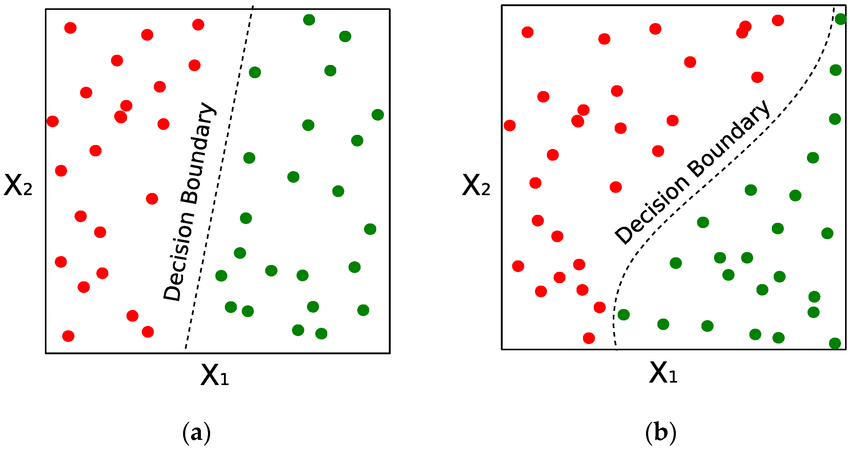
\includegraphics[width=0.9\linewidth]{./images/lin-non-lin.png}
    \caption{Example linear and non-linear decision boundaries on a two-dimensional graph. \cite{Duque2017}}
    \label{fig:linear-nonlinear}
\end{figure}
\subsection*{Linear Regression}
Linear regression is a very simple linear classifier that makes use of a straight line to separate classes. It estimates the relationship between a dependent variable, and one or more independent variables.

\begin{figure}[H]
    \centering
    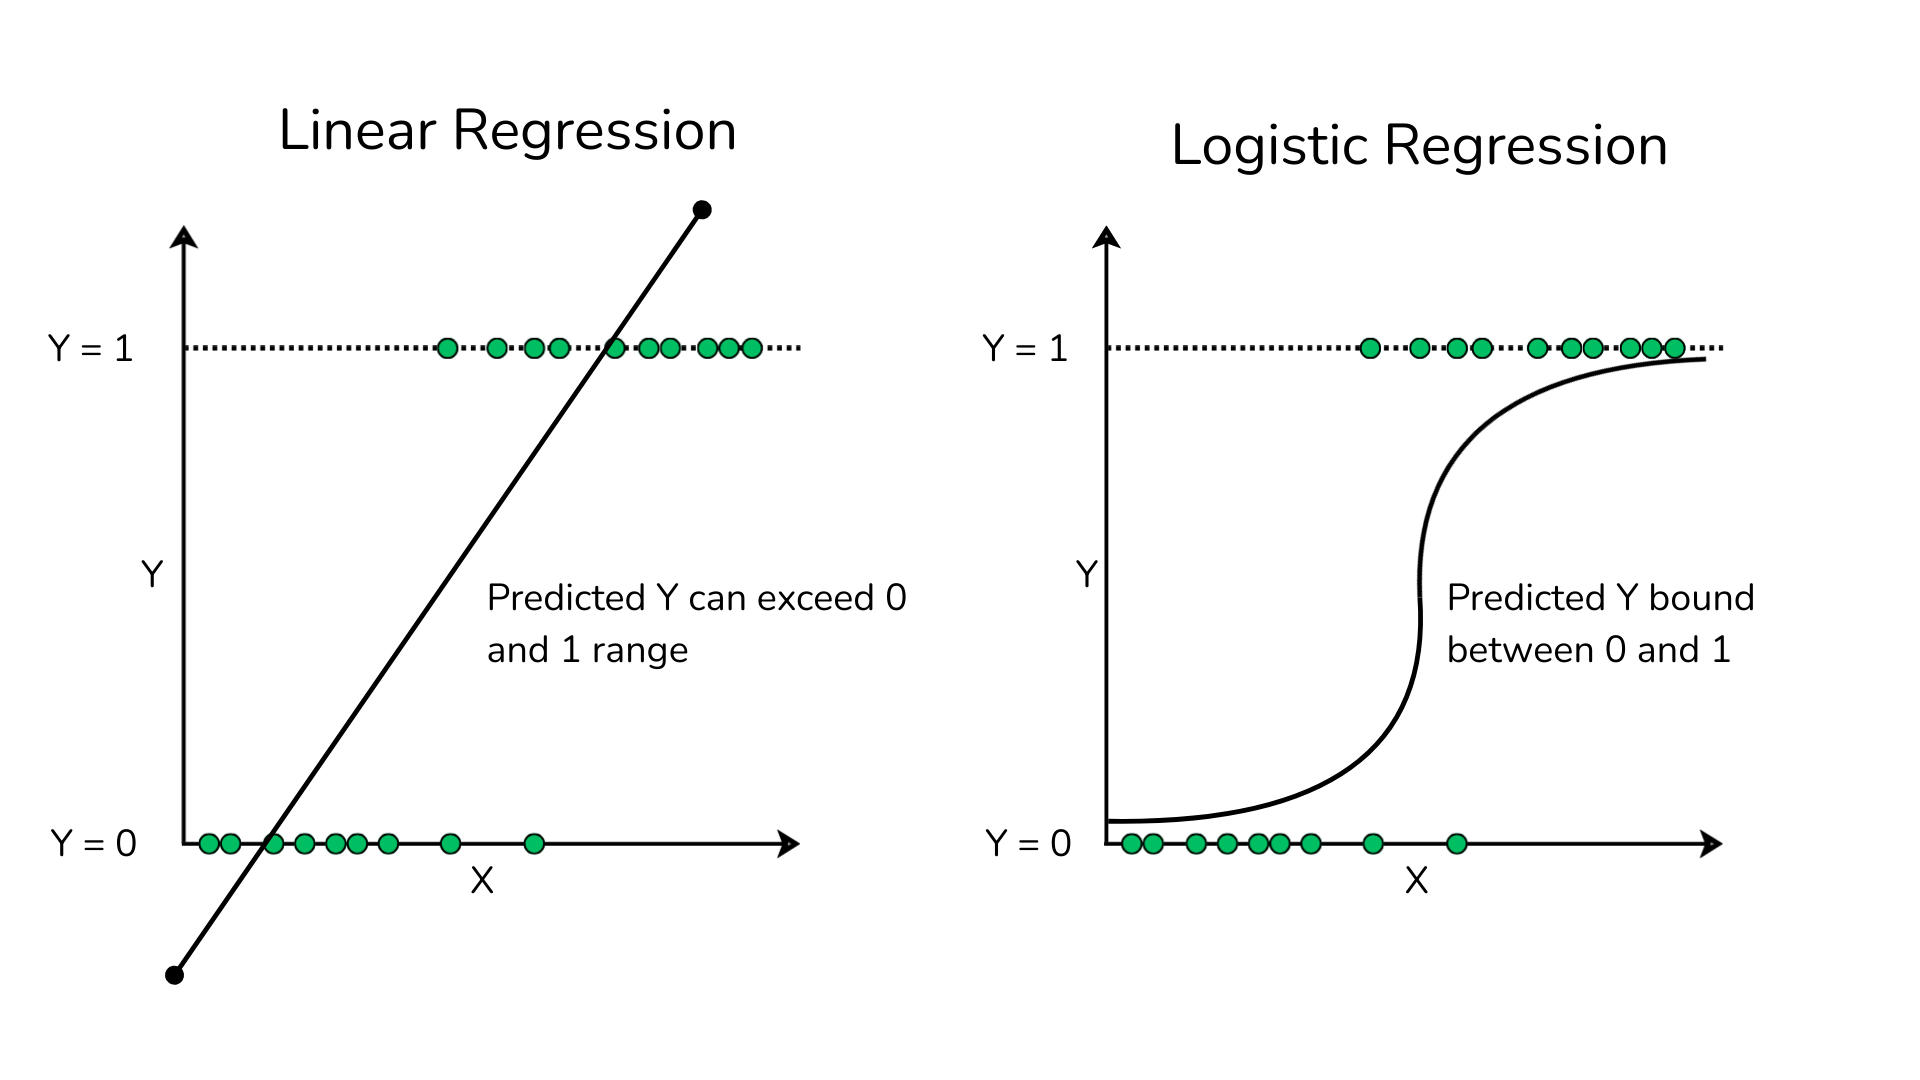
\includegraphics[width=0.9\linewidth]{./images/linear-logistic.png}
    \caption{Example of the Difference Between Linear and Logistic Regression}
    \label{fig:linear-vs-logistic}
\end{figure}

\subsection*{Logistic Regression}
Logistic regression is a linear classifier model that builds upon linear regression, mainly for use in binary classification problems, although there are multi-class implementations too. Logistic regression transforms the y values generated using linear regression into values bound between zero and one using the Sigmoid Function below.
\begin{equation*}
    \scalebox{2}[2]{\ensuremath{P = \frac{1}{1+e^{-x}}}}
\end{equation*}
Where \textit{P} is the probability of an event happening. Logistic regression is a simple model to understand, implement, and train, making it good for providing a baseline. However, due to the nature of its assumption of linearity between the dependent variable and the independent variables, this renders it unfit for non-linear relationships, which most reals world relationships are.\cite{osisanwo2017supervised}

\subsection*{K-Nearest Neighbours}
K-nearest neighbours is a simple to understand model that can be used for classification or \gls{regression} tasks. It calculates the distance of the training points from the new test point, taking the K nearest points to produce a prediction. For classification, the prediction will be the most frequent class among the K neighbours, and for regression it would be average of the values. The size of K is specified by the human, and needs to be adjusted until the value that works best for the specific usage is found. The means of measuring the best value can come from its accuracy, as well as the models run time and performance.

Since KNN calculates the distance from the test point to all the training points for every test point, it can be very computationally expensive as the number of training points grow, leading to slow predictions. Also, unlike other approaches that build models ahead of time, KNN doesn't 'learn' a model, so for every prediction, it requires going through the entire dataset, which makes it memory-intensive. Furthermore, KNN suffers from a phenomenon called the 'curse of dimensionality'. When the amount of dimensions (features per data point) increases, all training points become very far away from the test point, and the difference between the K neighbours is minimal in comparison to the overall distance from the test point. This makes the distance to neighbours less important, which for KNN, is its whole basis. \cite{osisanwo2017supervised}
\begin{figure}[H]
    \centering
    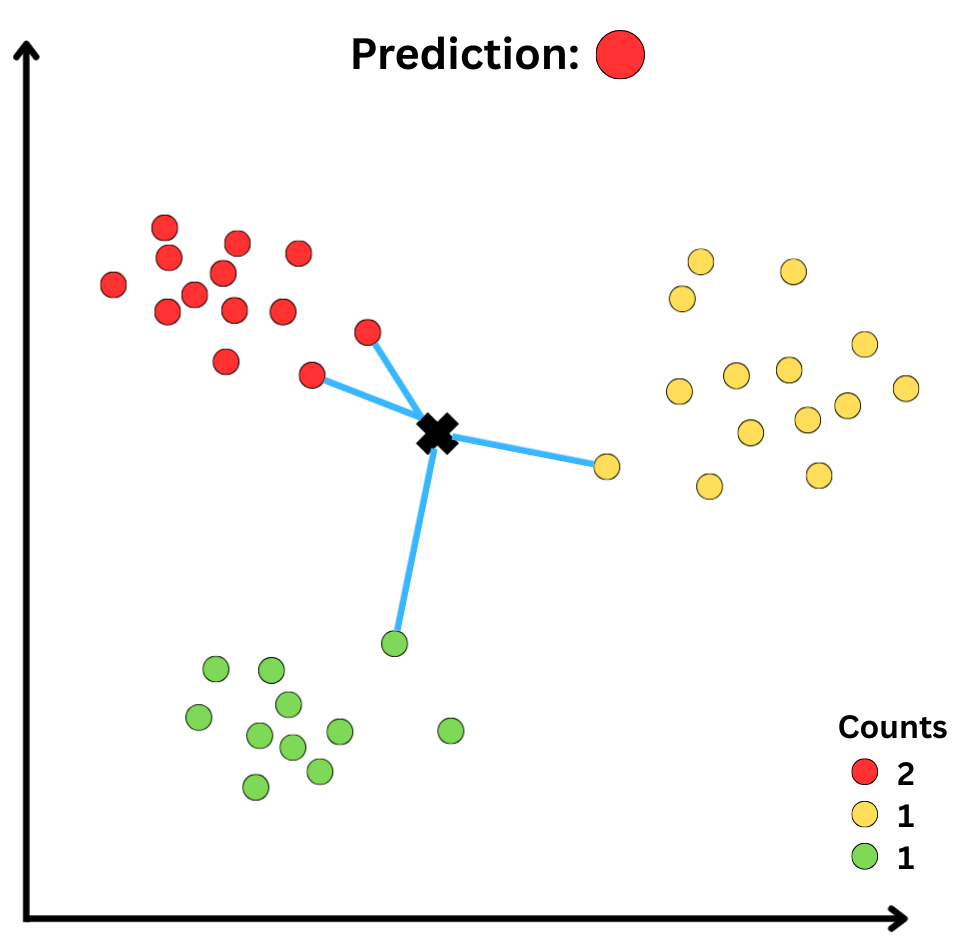
\includegraphics[width=0.6\linewidth]{./images/KNN figure.png}
    \caption{Figure Depicting 2D KNN Distances With K = 4}
    \label{fig:KNN}
\end{figure}
\subsubsection{Support Vector Machines (SVM)}
\begin{figure}[H]
    \centering
    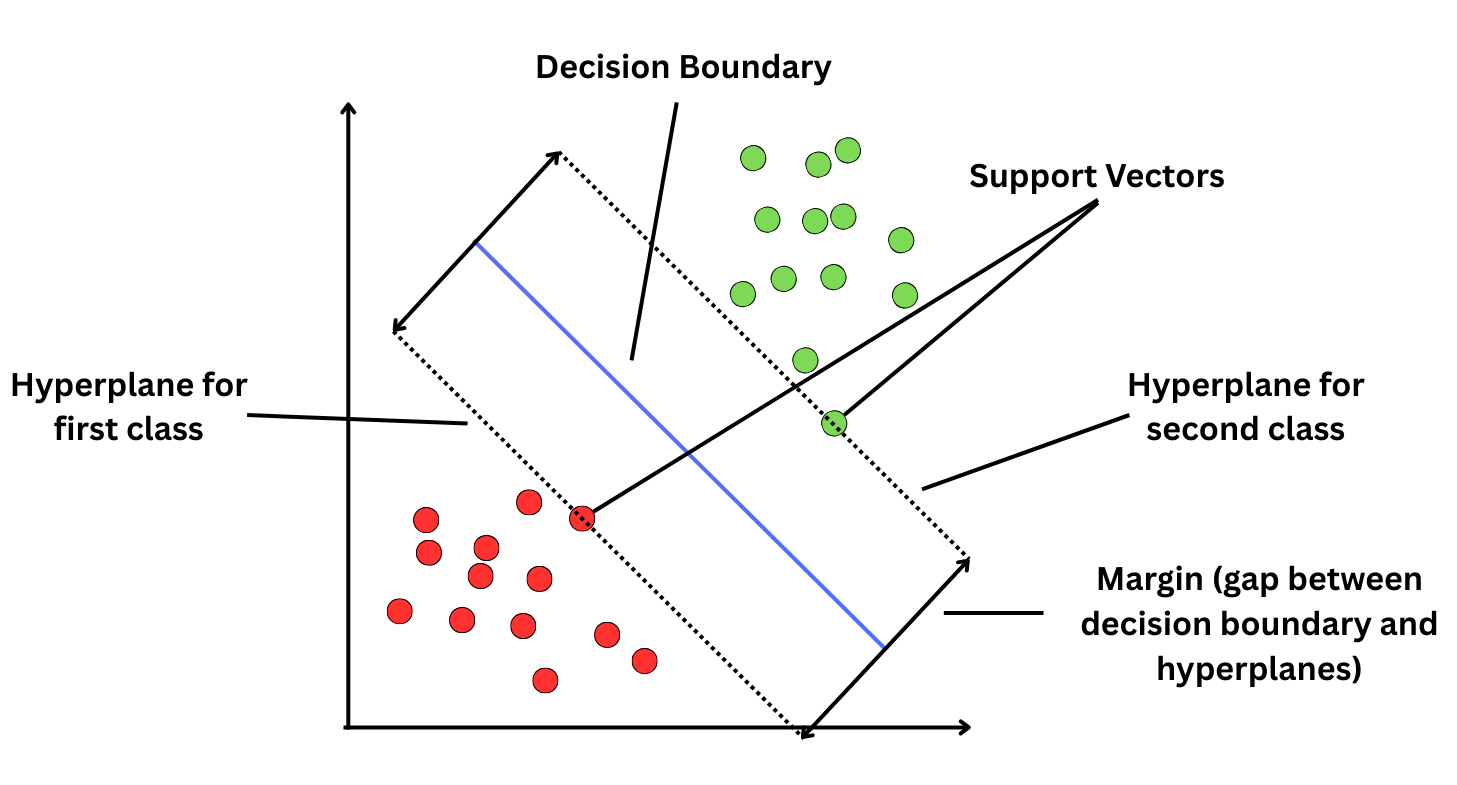
\includegraphics[width=0.9\linewidth]{./images/Support Vectors.png}
    \caption{Figure Depicting and SVM Example}
    \label{fig:SVM}
\end{figure}
SVMs work by finding the hyperplane that best separates the data points of different classes in a high-dimensional space. The optimal hyperplane maximises the margin between the nearest points of each class, known as the support vectors.

SVMs can handle both linear and non-linear data through the use of kernel functions, such as polynomial, radial basis function (RBF), or sigmoid kernels, which map the input data into higher dimensional spaces where it becomes linearly separable. SVMs are effective for high-dimensional datasets and can provide strong generalisation performance. However, they can be computationally expensive for large datasets, and selecting an appropriate kernel and tuning hyper-parameters such as C (regularisation) and gamma is necessary for good performance.\cite{osisanwo2017supervised}

\subsection*{Random Forest}
Random Forest is an \gls{ensemble} learning method based on decision trees, used for classification or regression. They work by constructing a large number of decision trees during training and outputting the majority vote for classification tasks or the average prediction for regression tasks.\footnote{For a visual explanation of random forest, watch \href{https://www.youtube.com/watch?v=v6VJ2RO66Ag}{this.}}

The key advantage of Random Forests is their ability to reduce \gls{overfitting} compared to a single decision tree, as each tree is trained on a random subset of the data and considers a random subset of features when splitting nodes. This introduces diversity among the trees, which improves overall performance. Random Forests are robust, can handle large datasets with many features, and provide feature importance metrics. However, they can become memory-intensive and slower to predict as the number of trees grows.\cite{osisanwo2017supervised}

\subsection*{Gradient Boosted Trees}
Gradient Boosted Trees (GBT) are another ensemble method that sequentially creates a decision tree, where each new tree is trained to correct the errors of the previous trees. This is done using gradient descent to minimise a chosen loss function, making the model highly accurate and capable of capturing complex patterns.

GBTs are powerful and often outperform simpler models like Logistic Regression or Random Forests on structured datasets. They are sensitive to hyper-parameter tuning, such as learning rate, number of trees, and tree depth, and can be prone to overfitting if not properly configured. They more computationally intensive than Random Forest, but they have the potential to be a lot more accurate too.\cite{osisanwo2017supervised}

\begin{figure}
    \centering
    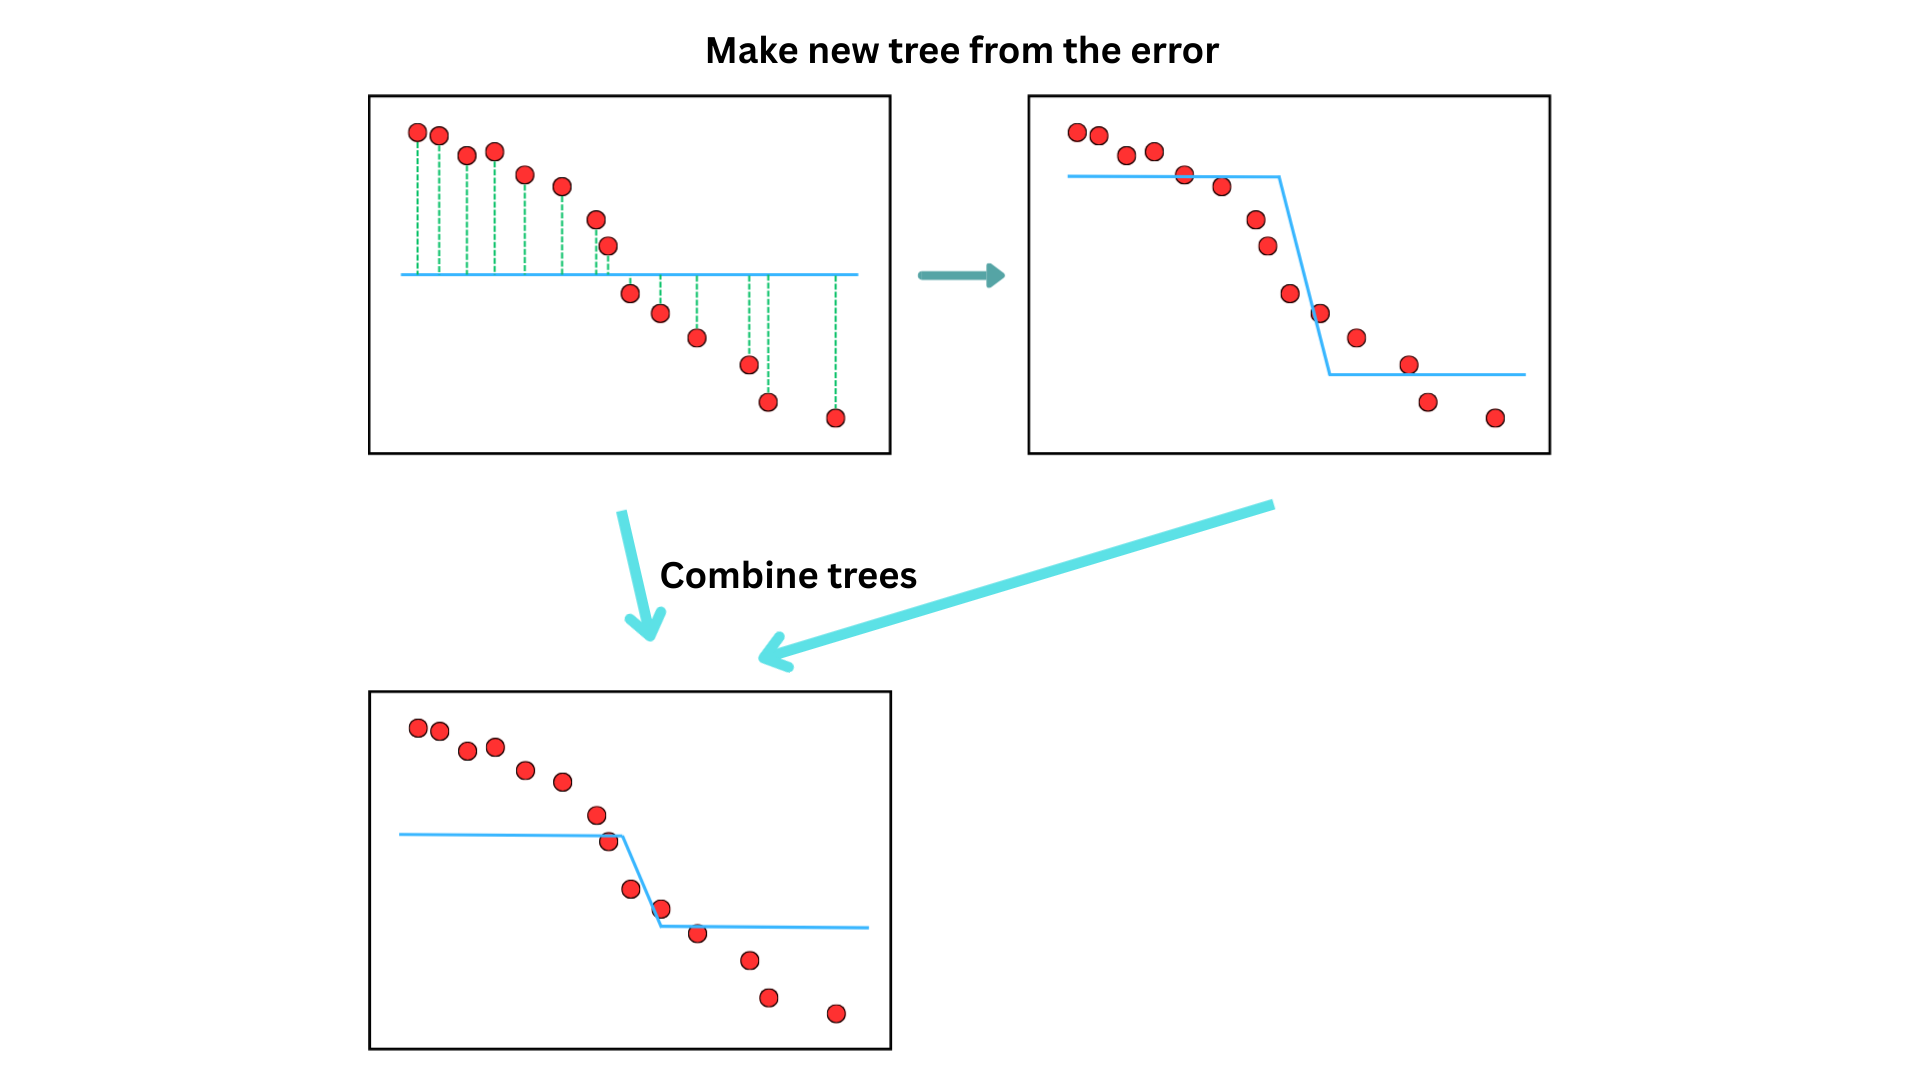
\includegraphics[width=0.9\linewidth]{./images/GBT1.png}
    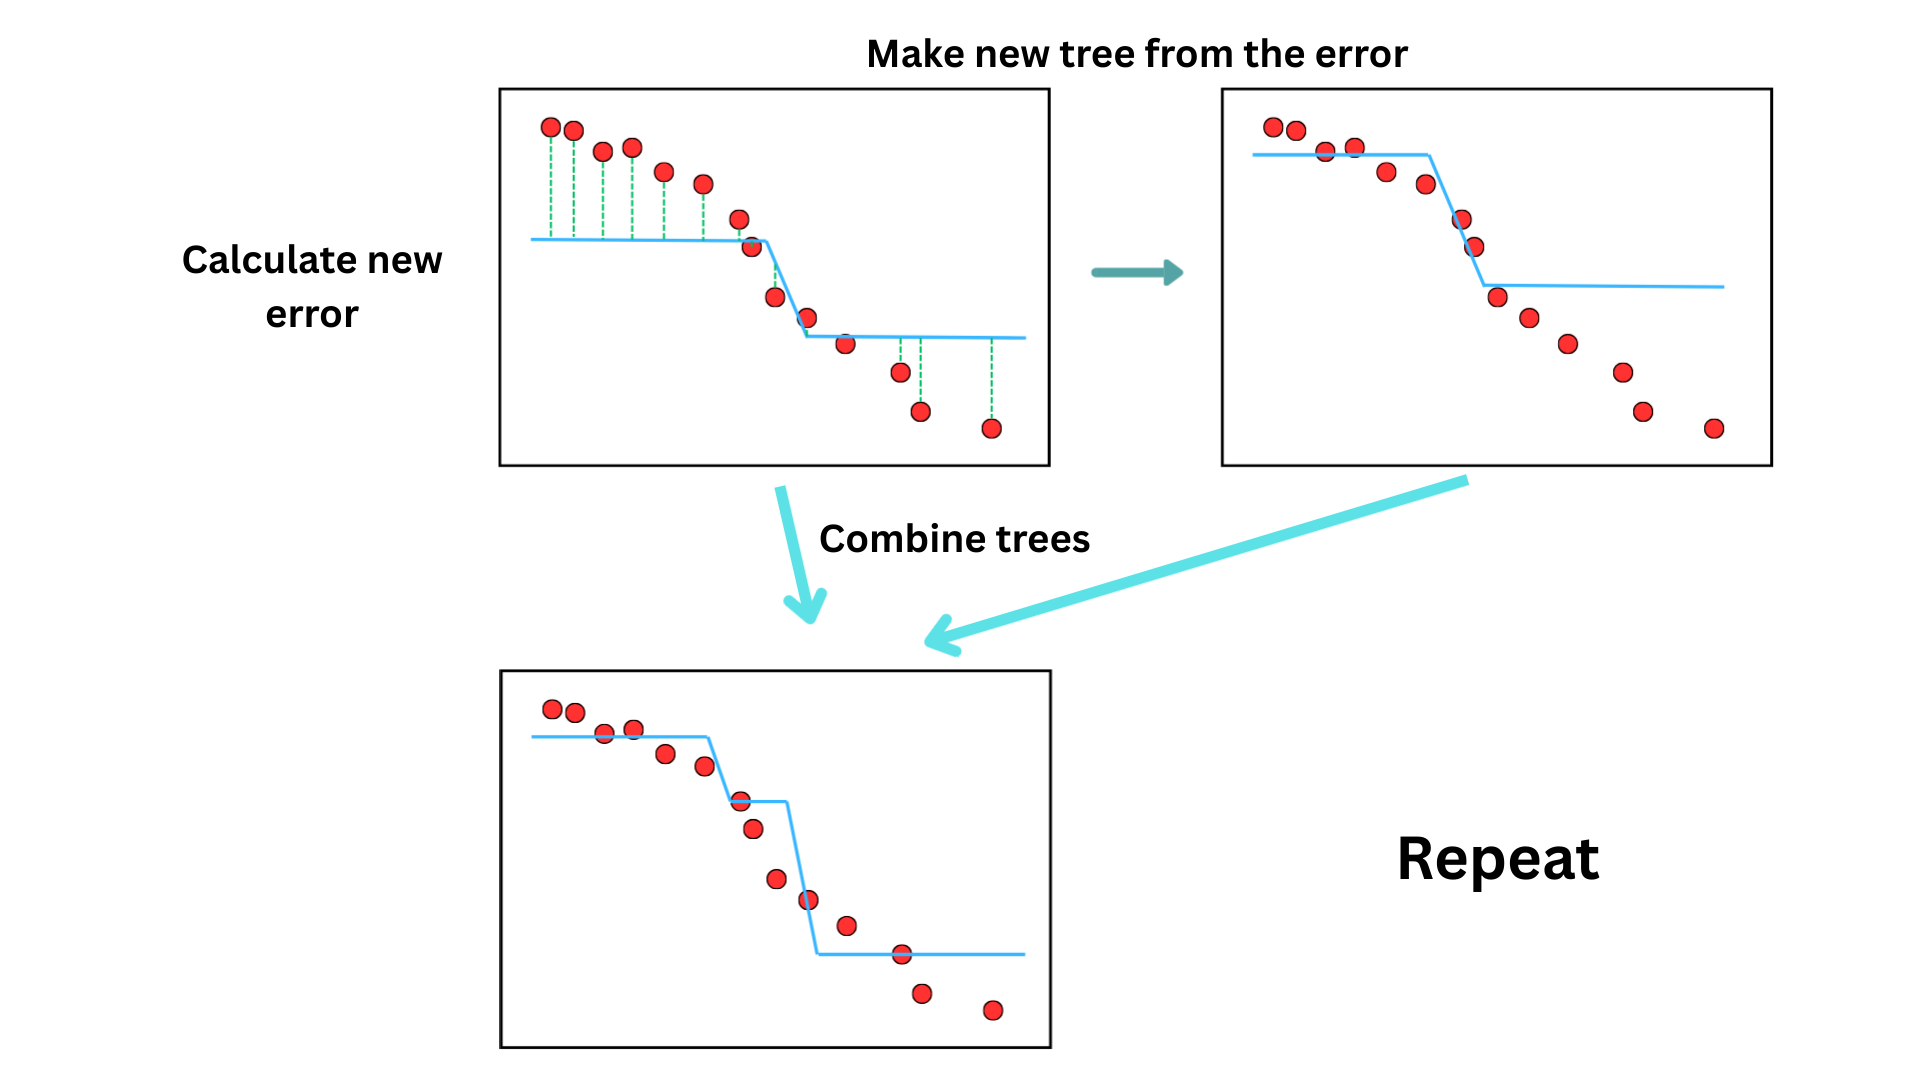
\includegraphics[width=0.9\linewidth]{./images/GBT2.png}
    \caption{Visual Example of Gradient Boosted Trees}
    \label{fig:GBT}
\end{figure}

\begin{table}[H]
    \centering
    \begin{tabular}{|l|>{\raggedright\arraybackslash}m{5cm}|>{\raggedright\arraybackslash}m{5cm}|}
        \hline
        \textbf{Model} & \textbf{Pros} & \textbf{Cons} \\ \hline

        \textbf{Linear Regression} &
        \vspace{4pt}\begin{itemize}[leftmargin=*,topsep=2pt,partopsep=0pt,parsep=0pt,itemsep=1pt]
            \item Simple to understand and implement
            \item Quick to train
            \item Provides a baseline for comparison
        \end{itemize}\vspace{4pt} &
        \vspace{4pt}\begin{itemize}[leftmargin=*,topsep=2pt,partopsep=0pt,parsep=0pt,itemsep=1pt]
            \item Assumes linear relationship between variables
            \item Poor performance on non-linear data
        \end{itemize}\vspace{4pt} \\ \hline

        \textbf{Logistic Regression} &
        \vspace{4pt}\begin{itemize}[leftmargin=*,topsep=2pt,partopsep=0pt,parsep=0pt,itemsep=1pt]
            \item Produces probabilistic outputs
            \item Easy to implement and interpret
            \item Works well as a baseline classifier
        \end{itemize}\vspace{4pt} &
        \vspace{4pt}\begin{itemize}[leftmargin=*,topsep=2pt,partopsep=0pt,parsep=0pt,itemsep=1pt]
            \item Assumes linear relationship between independent variables and log-odds
            \item Limited for complex non-linear relationships
        \end{itemize}\vspace{4pt} \\ \hline

        \textbf{K-Nearest Neighbours (KNN)} &
        \vspace{4pt}\begin{itemize}[leftmargin=*,topsep=2pt,partopsep=0pt,parsep=0pt,itemsep=1pt]
            \item Simple to understand and implement
            \item Can be used for classification or regression
            \item No training phase required
        \end{itemize}\vspace{4pt} &
        \vspace{4pt}\begin{itemize}[leftmargin=*,topsep=2pt,partopsep=0pt,parsep=0pt,itemsep=1pt]
            \item Computationally expensive for large datasets
            \item Memory-intensive (stores all training data)
            \item Performance degrades in high dimensions (curse of dimensionality)
        \end{itemize}\vspace{4pt} \\ \hline

        \textbf{Support Vector Machines (SVM)} &
        \vspace{4pt}\begin{itemize}[leftmargin=*,topsep=2pt,partopsep=0pt,parsep=0pt,itemsep=1pt]
            \item Effective in high-dimensional spaces
            \item Can handle non-linear data via kernels
            \item Strong generalisation performance
        \end{itemize}\vspace{4pt} &
        \vspace{4pt}\begin{itemize}[leftmargin=*,topsep=2pt,partopsep=0pt,parsep=0pt,itemsep=1pt]
            \item Computationally expensive for large datasets
            \item Requires careful selection of kernel and hyper-parameters
        \end{itemize}\vspace{4pt} \\ \hline

        \textbf{Random Forest} &
        \vspace{4pt}\begin{itemize}[leftmargin=*,topsep=2pt,partopsep=0pt,parsep=0pt,itemsep=1pt]
            \item Reduces overfitting compared to single decision trees
            \item Handles large datasets and many features
            \item Provides feature importance metrics
            \item Robust and relatively easy to tune
        \end{itemize}\vspace{4pt} &
        \vspace{4pt}\begin{itemize}[leftmargin=*,topsep=2pt,partopsep=0pt,parsep=0pt,itemsep=1pt]
            \item Can become memory-intensive
            \item Slower prediction with many trees
        \end{itemize}\vspace{4pt} \\ \hline

        \textbf{Gradient Boosted Trees (GBT)} &
        \vspace{4pt}\begin{itemize}[leftmargin=*,topsep=2pt,partopsep=0pt,parsep=0pt,itemsep=1pt]
            \item High predictive accuracy
            \item Captures complex patterns
            \item Often outperforms simpler models
        \end{itemize}\vspace{4pt} &
        \vspace{4pt}\begin{itemize}[leftmargin=*,topsep=2pt,partopsep=0pt,parsep=0pt,itemsep=1pt]
            \item Computationally intensive
            \item Sensitive to hyper-parameter tuning
            \item Can overfit if not properly \gls{regularised}
        \end{itemize}\vspace{4pt} \\ \hline

    \end{tabular}
    \caption{Pros and cons of each machine learning model described.}
    \label{tab:MLModelProsCons}
\end{table}
\noindent
Based on the pros and cons of each classification algorithm, I have chosen to use Random Forest initially to quickly establish a baseline accuracy, and then I will implement Gradient Boosted Trees (GBT) to improve predictive performance, taking care to properly tune hyper-parameters and apply \gls{regularisation} to prevent overfitting.